\documentclass[../main.tex]{subfiles}
\begin{document}

\section{Starting Source Golf}
This section explains how to start once the board is built, and the players have learned some of he basics above. 

\subsection{Determining Turn Order}
Players will first determine the turn order for hitting their ball and then start the game. 

Roll a D20 for each player. The player with the highest roll will choose their ball first and play first. The order of other players continues in descending order. If there are any ties, re-roll the tied rolls to determine the order. 

For the rest of the round, the player whose ball is furthest from the hole will be next in turn order. 

\textit{Note: This means players can go multiple times in a row if they continue to be the farthest from the hole.} 

For more rounds or holes, the player with the lowest score will be the first to play. 

\section{Playing Source Golf: Player Turn}
\begin{enumerate}
\item Chose a starting hex from the tee box. Place the ball for the first hit. 
\item Point the front arrow down a line of hexes for the ball to travel down. 

\begin{figure}[h]
    \centering
    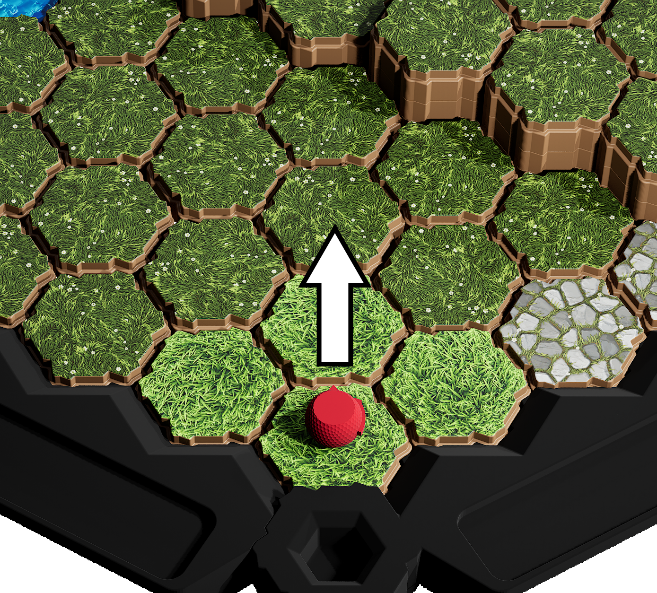
\includegraphics[width=0.75\linewidth]{chapters//startingsourcegolf/Source Golf FrontArrowDirectional.png}
\end{figure}

\item Flip the ball so the side arrow is on the left or right, to determine the flight path of the ball (this emulates a slice or draw). 
\item Choose a die from one of the following to act as your club and roll it: 
    
\begin{TimeStrikeTable}[header=Dice equivalent to Clubs]{XX}
    \textbf{Dice}  & \textbf{Clubs} \\
    D20  & Driver \\
    D12  & Wood \\
    D8  & Iron \\
    D6  & Wedge \\
    D4  & Putter \\
\end{TimeStrikeTable}

\item Using the number rolled, pick up that number of dice from the set of 20D6 and roll them. For example, you choose a D8 (iron) and roll a 6. Choose 6 D6 dice from the pile and roll them. 
\item Now you will sort your rolled D6s into three groups. 
\begin{enumerate}
\item 1's - Set these aside. These represent the amount of spin you put on the ball. For each 1 rolled, move the ball one hex in the direction the curved arrow is pointing toward. For example: if the curved arrow is on the right, move the ball to the hex right of the direction the front arrow is aimed at. \textit{Note: Do not turn the ball in the process, keep the front arrow pointing in the same direction.}

\begin{figure}[h]
    \centering
    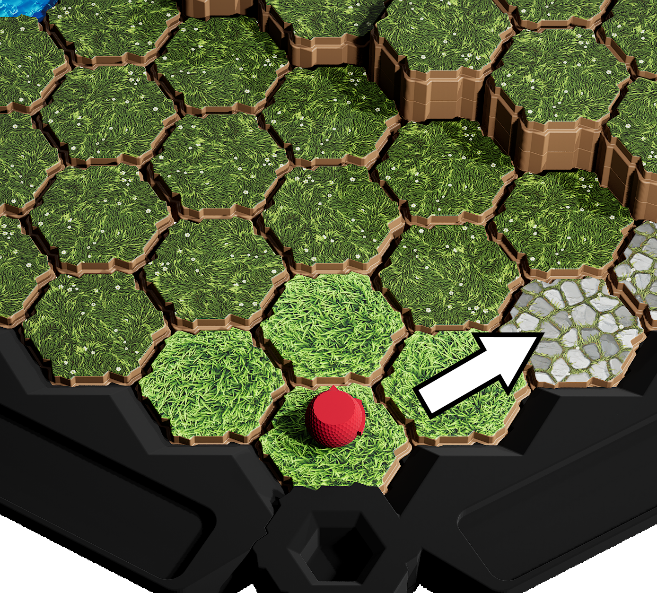
\includegraphics[width=0.75\linewidth]{chapters//startingsourcegolf/Source Golf CurvedArrowDirectional.png}   
\end{figure}

\item 2 - 5 - The total number of dice that show a value of 2 - 5 represent how hard you actually hit the ball or your power. Move the ball one hex straight forward for each dice showing 2 - 5, where the front arrow is pointing.  For example, you roll six dice, and four of them show a value between two and five,  your hit power is four hexes forward. 

\item 6's - Set these aside. These represent the wind resistance. For each 6 rolled, move the ball that many hexes to the opposite side of the curved arrow. For example: If the curved arrow is on the right, move the ball to the hex left of the front arrow is aimed at. 

\begin{figure}[h]
    \centering
    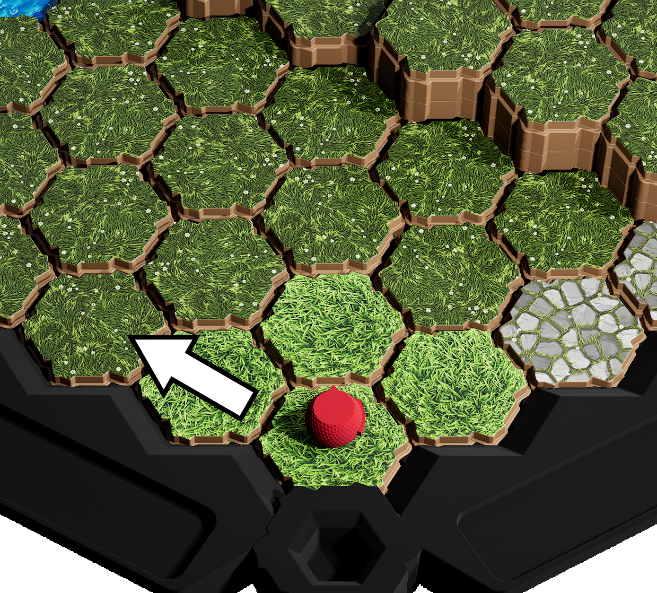
\includegraphics[width=1\linewidth]{chapters//startingsourcegolf/SourceGolfBallWindResistance.png} 
\end{figure}

\end{enumerate}
\item Apply the dice rolls for the forward movement, spin, and wind resistance to determine where the ball lands and move it accordingly. 
   
\end{enumerate}

From the ball's current location, repeat steps 2 through 7. Each time the process is repeated, a player adds 1 stroke to their score. Continue until a player lands the golf ball onto the flag or in the putting green. 
\end{document}
